\documentclass[a4paper, 11pt]{article}
\usepackage[cpp]{mypackage}
\usepackage{amsmath}
\usepackage{graphicx}
\usepackage{geometry}
\usepackage{listings}
\geometry{scale=0.8}
\usepackage{hyperref}

\title{
\normalfont \normalsize
\textsc{School of Data and Computer Science, Sun Yat-sen University} \\ [25pt] %textsc small capital letters
\rule{\textwidth}{0.5pt} \\[0.4cm] % Thin top horizontal rule
\huge  E08 FF Planner(2)\\ % The assignment title
\rule{\textwidth}{2pt} \\[0.5cm] % Thick bottom horizontal rule
\author{17341015 Hongzheng Chen}
\date{\normalsize\today}
}

\lstset{language=lisp}

\begin{document}
\maketitle
\tableofcontents
\newpage
\section{Boxman Game}
If you don't know how to play the boxman game, you should open \texttt{BoxMan.zip} and click \texttt{BoxMan.exe} to have a try.  You can also choose the level of the game to challenge yourselves. There are five cases choosed from level 1, 10, 30, 40, 50 in the following figures.

You can model the location information based on rectangular coordinates as mapped out in Figure 3. For example, we denote by P13 the position (1,3). The calculated action sequence can be like this: \texttt{MOVE P12 P13, PUSH BOX1 P14 P15...},which means the guy runs from position (1,2) to position (1,3), and push the box1 from position (1,4) to position (1,5). However, this is only a very simple and intuitive approach to representing the actions and positions. If you have any other better methods, you can have a try.

Please solve the boxman game by using FF planner. You should hand in 2 files, including a domain file (\texttt{boxman\_domain.pddl}) and data file (\texttt{boxman5.pddl}).
\begin{figure}[h]
  \centering
  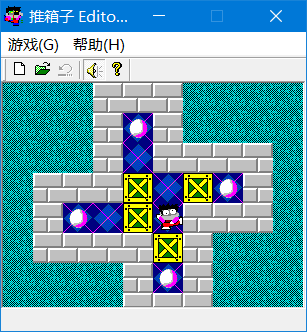
\includegraphics[width=6cm]{fig/case1}
  \qquad
  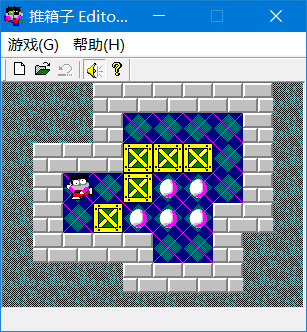
\includegraphics[width=6cm]{fig/case2}
  \caption{Boxman case1 (level 1) and case2 (level 10)}
\end{figure}
\begin{figure}[h]
  \centering
  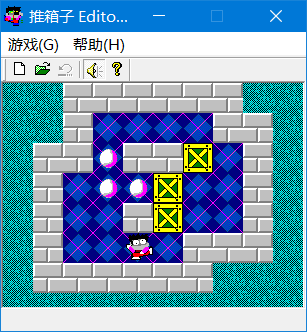
\includegraphics[width=6cm]{fig/case3}
  \qquad
  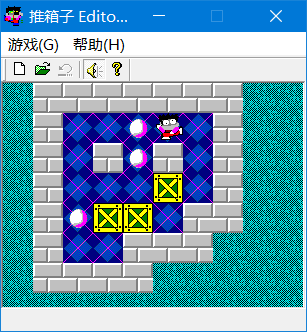
\includegraphics[width=6cm]{fig/case4}
  \caption{Boxman case3 (level 30) and case4 (level 40)}
\end{figure}
\begin{figure}[h]
  \centering
  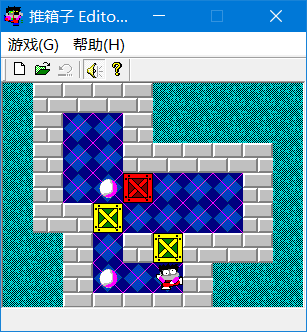
\includegraphics[width=6cm]{fig/case5}
  \qquad
  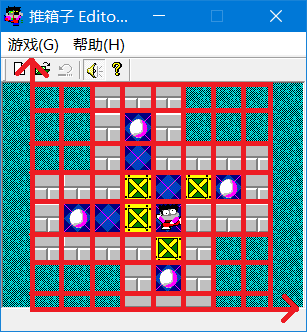
\includegraphics[width=6cm]{fig/model}
  \caption{Boxman case5 (level 50) and modelling}
\end{figure}

\section{Notes}
\par Please send \textbf{E08\_YourNumber.zip} which should contain the codes(\textbf{ai\_201901@foxmail.com}).

\section{Codes \& Results}
Codes are listed below.
I define \verb'inc' and \verb'dec' to do simple calculation judging whether two grids are adjacent.
Actions of four directions are defined representively.
And the final goal is simply defined as several \verb'box(x,y)' positions, i.e. requesting boxes at some grid $(x,y)$.

The 1st, 3th, 4th, 5th problem are solved on the online planner\footnote{\url{http://editor.planning.domains/}}.
The 2nd one is solved by Metric-FF planner v2.1\footnote{\url{https://fai.cs.uni-saarland.de/hoffmann/metric-ff.html}} on my local system.

For the planning results, please refer to \verb'Plan (X).txt'.
\begin{lstlisting}[title=boxman\_domain.pddl]
(define (domain boxman)

(:requirements :strips :typing :equality)

(:predicates
    (inc ?p ?p1)
    (dec ?p ?p1)
    (empty ?x ?y)
    (box ?x ?y)
    (pos ?x ?y)
)

(:action move-down
    :parameters (?x ?y ?yTo)
    :precondition (and
        (pos ?x ?y)
        (dec ?y ?yTo)
        (empty ?x ?yTo)
        )
    :effect (and
        (not (pos ?x ?y))
        (pos ?x ?yTo)
        (not (empty ?x ?yTo))
        (empty ?x ?y)
        )
)

(:action move-up
    :parameters (?x ?y ?yTo)
    :precondition (and
        (pos ?x ?y)
        (inc ?y ?yTo)
        (empty ?x ?yTo)
        )
    :effect (and
        (not (pos ?x ?y))
        (pos ?x ?yTo)
        (not (empty ?x ?yTo))
        (empty ?x ?y)
        )
)

(:action move-left
    :parameters (?x ?y ?xTo)
    :precondition (and
        (pos ?x ?y)
        (dec ?x ?xTo)
        (empty ?xTo ?y)
        )
    :effect (and
        (not (pos ?x ?y))
        (pos ?xTo ?y)
        (not (empty ?xTo ?y))
        (empty ?x ?y)
        )
)

(:action move-right
    :parameters (?x ?y ?xTo)
    :precondition (and
        (pos ?x ?y)
        (inc ?x ?xTo)
        (empty ?xTo ?y)
        )
    :effect (and
        (not (pos ?x ?y))
        (pos ?xTo ?y)
        (not (empty ?xTo ?y))
        (empty ?x ?y)
        )
)

; right x+ up y+
(:action push-down
    :parameters (?x ?y ?yBox ?yTo)
    :precondition (and
        (pos ?x ?y)
        (dec ?y ?yBox)
        (dec ?yBox ?yTo)
        (box ?x ?yBox)
        (empty ?x ?yTo)
        )
    :effect (and
        (not (pos ?x ?y))
        (pos ?x ?yBox)
        (not (box ?x ?yBox))
        (box ?x ?yTo)
        (not (empty ?x ?yTo))
        (empty ?x ?y)
        )
)

(:action push-up
    :parameters (?x ?y ?yBox ?yTo)
    :precondition (and
        (pos ?x ?y)
        (inc ?y ?yBox)
        (inc ?yBox ?yTo)
        (box ?x ?yBox)
        (empty ?x ?yTo)
        )
    :effect (and
        (not (pos ?x ?y))
        (pos ?x ?yBox)
        (not (box ?x ?yBox))
        (box ?x ?yTo)
        (not (empty ?x ?yTo))
        (empty ?x ?y)
        )
)

(:action push-left
    :parameters (?x ?y ?xBox ?xTo)
    :precondition (and
        (pos ?x ?y)
        (dec ?x ?xBox)
        (dec ?xBox ?xTo)
        (box ?xBox ?y)
        (empty ?xTo ?y)
        )
    :effect (and
        (not (pos ?x ?y))
        (pos ?xBox ?y)
        (not (box ?xBox ?y))
        (box ?xTo ?y)
        (not (empty ?xTo ?y))
        (empty ?x ?y)
        )
)

(:action push-right
    :parameters (?x ?y ?xBox ?xTo)
    :precondition (and
        (pos ?x ?y)
        (inc ?x ?xBox)
        (inc ?xBox ?xTo)
        (box ?xBox ?y)
        (empty ?xTo ?y)
        )
    :effect (and
        (not (pos ?x ?y))
        (pos ?xBox ?y)
        (not (box ?xBox ?y))
        (box ?xTo ?y)
        (not (empty ?xTo ?y))
        (empty ?x ?y)
        )
)

)
\end{lstlisting}

\begin{lstlisting}[title=boxman1.pddl]
  (define (problem prob1)
  (:domain boxman)
  (:objects p1 p2 p3 p4 p5 p6)
  (:init
      (inc p1 p2)
      (inc p2 p3)
      (inc p3 p4)
      (inc p4 p5)
      (inc p5 p6)
      (dec p6 p5)
      (dec p5 p4)
      (dec p4 p3)
      (dec p3 p2)
      (dec p2 p1)
      (pos p4 p3)
      (empty p1 p3)
      (empty p2 p3)
      (empty p3 p5)
      (empty p3 p6)
      (empty p4 p4)
      (empty p6 p4)
      (empty p4 p1)
      (box p4 p2)
      (box p3 p3)
      (box p3 p4)
      (box p5 p4)
  )
  (:goal (and
      (box p4 p1)
      (box p1 p3)
      (box p6 p4)
      (box p3 p6)
      )
  )
)
\end{lstlisting}

% ./ff -p . -o boxman_domain.pddl -f boxman2.pddl -s 0
\begin{lstlisting}[title=boxman2.pddl]
  (define (problem prob2)
  (:domain boxman)
  (:objects p1 p2 p3 p4 p5 p6)
  (:init
      (inc p1 p2)
      (inc p2 p3)
      (inc p3 p4)
      (inc p4 p5)
      (inc p5 p6)
      (dec p6 p5)
      (dec p5 p4)
      (dec p4 p3)
      (dec p3 p2)
      (dec p2 p1)
      (pos p1 p3)
      (empty p1 p2)
      (empty p2 p3)
      (empty p3 p2)
      (empty p3 p5)
      (empty p4 p1)
      (empty p4 p2)
      (empty p4 p3)
      (empty p4 p5)
      (empty p5 p1)
      (empty p5 p2)
      (empty p5 p3)
      (empty p5 p5)
      (empty p6 p3)
      (empty p6 p4)
      (empty p6 p5)
      (box p2 p2)
      (box p3 p3)
      (box p3 p4)
      (box p4 p4)
      (box p5 p4)
  )
  (:goal (and
      (box p3 p2)
      (box p4 p3)
      (box p5 p3)
      (box p4 p2)
      (box p5 p2)
      )
  )
)
\end{lstlisting}

\begin{lstlisting}[title=boxman3.pddl]
  (define (problem prob3)
  (:domain boxman)
  (:objects p1 p2 p3 p4 p5 p6)
  (:init
      (inc p1 p2)
      (inc p2 p3)
      (inc p3 p4)
      (inc p4 p5)
      (inc p5 p6)
      (dec p6 p5)
      (dec p5 p4)
      (dec p4 p3)
      (dec p3 p2)
      (dec p2 p1)
      (pos p3 p1)
      (empty p1 p1)
      (empty p1 p2)
      (empty p1 p3)
      (empty p2 p1)
      (empty p2 p2)
      (empty p2 p3)
      (empty p2 p4)
      (empty p2 p5)
      (empty p3 p3)
      (empty p3 p5)
      (empty p4 p1)
      (empty p4 p5)
      (empty p5 p2)
      (empty p5 p3)
      (empty p5 p5)
      (empty p6 p2)
      (empty p6 p3)
      (empty p6 p4)
      (box p4 p2)
      (box p4 p3)
      (box p5 p4)
  )
  (:goal (and
      (box p2 p4)
      (box p2 p3)
      (box p3 p3)
      )
  )
)
\end{lstlisting}

\begin{lstlisting}[title=boxman4.pddl]
  (define (problem prob4)
  (:domain boxman)
  (:objects p1 p2 p3 p4 p5)
  (:init
      (inc p1 p2)
      (inc p2 p3)
      (inc p3 p4)
      (inc p4 p5)
      (dec p5 p4)
      (dec p4 p3)
      (dec p3 p2)
      (dec p2 p1)
      (pos p4 p5)
      (empty p1 p1)
      (empty p1 p2)
      (empty p1 p3)
      (empty p1 p4)
      (empty p1 p5)
      (empty p2 p1)
      (empty p2 p3)
      (empty p2 p5)
      (empty p3 p3)
      (empty p3 p4)
      (empty p3 p5)
      (empty p4 p2)
      (empty p4 p5)
      (empty p5 p3)
      (empty p5 p4)
      (empty p5 p5)
      (box p2 p2)
      (box p3 p2)
      (box p4 p3)
  )
  (:goal (and
      (box p1 p2)
      (box p3 p4)
      (box p3 p5)
      )
  )
)
\end{lstlisting}

\begin{lstlisting}[title=boxman5.pddl]
  (define (problem prob5)
  (:domain boxman)
  (:objects p1 p2 p3 p4 p5 p6)
  (:init
      (inc p1 p2)
      (inc p2 p3)
      (inc p3 p4)
      (inc p4 p5)
      (inc p5 p6)
      (dec p6 p5)
      (dec p5 p4)
      (dec p4 p3)
      (dec p3 p2)
      (dec p2 p1)
      (pos p4 p1)
      (empty p1 p4)
      (empty p1 p5)
      (empty p1 p6)
      (empty p2 p1)
      (empty p2 p2)
      (empty p2 p4)
      (empty p2 p5)
      (empty p2 p6)
      (empty p3 p1)
      (empty p3 p3)
      (empty p3 p3)
      (empty p4 p3)
      (empty p4 p4)
      (empty p5 p3)
      (empty p5 p4)
      (empty p6 p3)
      (empty p6 p4)
      (box p2 p3)
      (box p3 p4)
      (box p4 p2)
  )
  (:goal (and
      (box p2 p1)
      (box p2 p4)
      (box p3 p4)
      )
  )
)
\end{lstlisting}

\end{document}